\section{The Cantor Set}

\begin{definition}
    We define the \textbf{Cantor set} $\Cc$ to be the intersection
    \begin{equation*}
        \Cc=\bigcap{C_k}
    \end{equation*}
    where $\{C_k\}$ is a descending collection of closed sets in which for each
    $k \in \Z^+$,  $\C_k$ is the disjoint union of  $2^k-1$ closed intervals
    each of length  $\frac{1}{3^k}$.
\end{definition}

\begin{theorem}\label{8.7.1}
    The Cantor set is a closed and uncountable set of measure $m(\Cc)=0$.
\end{theorem}
\begin{proof}
    Since $\Cc$ is an arbitrary intersection of closed sets in  $\R$,  $\Cc$ is
    closed in  $\R$. Moreover, by the definition of each  $C_k$,  $C_k$ is
    measurable and
    \begin{equation*}
        m(C_k)=\Big{(} \frac{2}{3} \Big{)}^k \text{ for each } k \in \Z^+
    \end{equation*}
    Then $\Cc$ is also measurable, and we have by monotonicity of the Lebesgue
    measure
    \begin{equation*}
        m(\Cc) \leq m(C_k)=\Big{(} \frac{2}{3} \Big{)}^k
    \end{equation*}
    Taking $k \xrightarrow{} \infty$, gives us that $m(\Cc)=0$.

    Now, suppose that $\Cc$ is countable, and let $\Cc=\{c_k\}$ be an
    enumeration of $\Cc$. Now, one of the disjoint intervals whose union is
    $C_1$ fails to contain $c_1$; call it $F_1$. Proceeding, one of the disjoint
    intervals whose union is $F_1$ fails to contain $c_2$; call it $F_2$.
    Proceeding inductively, we get a descending collection $\{F_k\}$ of closed
    sets, for which $c_k \notin F_k$ for each  $k \in \Z^+$. Now, by the nested
    set theorem, the intersection
    \begin{equation*}
        F=\bigcap{F_k}
    \end{equation*}
    is nonempty. Moreover, $F \subseteq \Cc$. This implies that there is an
    element $x \in \Cc$ which is not equal to any $c_k$; but $\{c_k\}$ is an
    enumeration of $\Cc$, which is absurd! Therefore, $\Cc$ fails to be
    countable.
\end{proof}

\begin{definition}
    Let $\Cc$ be the Cantor set, and define  $U_k$ such that
    $C_k=\com{[0,1]}{U_k}$, and define $\Uc=\bigcup{U_k}$; so that $[0,1]=\Cc
    \cup \Uc$. Fix $k \in \Z^+$ and define
    \begin{equation*}
        \phi:U_k \xrightarrow{} \R
    \end{equation*}
    to be the increasing function which is constant on each of the $2^k-1$
    intervals of  $U_k$, and whose image is
    \begin{equation*}
        \phi([0,1])=
        \Big{\{} \frac{1}{2^k}, \frac{2}{2^k}, \dots, \frac{2^k-1}{2^k} \Big{\}}
    \end{equation*}
    We define the \textbf{Cantor-Lebesgue function} to be the extension $\Phi$
    of  $\phi$ to  $[0,1]$; defined in terms of $\Cc$ to be
    \begin{equation*}
        \Phi(0)=\phi(0)=0 \text{ and }
        \Phi(x)=\sup{\{\phi(t): t \in \Uc \cap [0,x] \}} \text{ for all }
        x \in \com{\Cc}{\{0\}}
    \end{equation*}
\end{definition}

\begin{figure}[h]
    \centering
    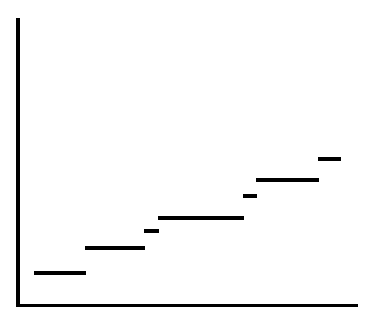
\includegraphics[scale=0.5]{Figures/chapter8/cantor_lebesgue_function.eps}
    \caption{The Canotr Lebesgue Function on $U_3$.}
    \label{figure_8.1}
\end{figure}

\begin{theorem}\label{8.7.2}
    The Cantor-Lebesgue function is an increasing continuous finction mapping
    $[0,1]$ onto $[0,1]$, and differentiable on $\Uc$ with
    \begin{equation*}
        \Phi'(x)=0 \text{ on } \Uc \text{ where } m(\Uc)=1
    \end{equation*}
\end{theorem}
\begin{proof}
    Since $\phi$ is an increasing fucntion, and  $\Phi$ is the extension of
    $\phi$ to  $[0,1]$, then $\Phi$ must also be increasing. Now,  $\phi$ is
    continuous at each point of  $\Uc$, since it is constant on each  $U_k$.
    Now, consider  $x_0 \in \Cc$ with $x_0 \neq 0,1$. Then $x_0 \notin U_k$ for
    all $k \in \Z^+$. So for  $k$ large enought,  $x_0$ lies in between
    consecutive intervals of $U_k$. Choose  $a_k$ to be the lowerbound of the
    lower interval, and  $b_k$ the upperbound of the upper interval. Then by
    definition of  $\phi$, we get
    \begin{equation*}
        a_k<x_0<b_k \text{ and } \phi(b_k)-\phi(a_k)=\frac{1}{2^k}
    \end{equation*}
    Since $k$ is arbitrarily large, $\Phi$ fails to have a jump discontinuity at
     $x_0$, which is the only possible discontinuity it can have. Therefore
     $\Phi$ is continuous at  $x_0$. A similar argument shows that $\Phi$ is
     continuous at $x_0=0,1$.

     Now, since $\phi$ is constant on each  $U_k$,  $\phi$ is differentiable on
      $U_k$ and has  $\phi'=0$ on each  $U_k$, hence  $\phi'=0$ on $\Uc$. Since
      $m(\Cc)=0$ and $[0,1]=\Cc \cup \Uc$, then $m(\Uc)=1$. Since $\Phi$ is an
      extension, we get that
      \begin{equation*}
          \Phi'=0 \text{ on } \Uc \text{ where } m(\Uc)=1
      \end{equation*}

      Finally, since $\Phi(0)=0$ and $\Phi(1)=1$, and $\Phi$ is increasing, by
      the intermediate value theorem $\Phi([0,1])=[0,1]$.
\end{proof}

\begin{lemma}\label{8.7.3}
    Let $\Phi$ be the Cantor-Lebesgue function, and define $\Psi:[0,1]
    \xrightarrow{} \R$ by
    \begin{equation*}
        \Psi(x)=\Phi(x)+x \text{ for all } x \in [0,1]
    \end{equation*}
    Then $\Psi$ is strictly increasing, and maps $[0,1]$ onto $[0,2]$. Moreover,
    $\Psi$ maps the Cantor set onto a set of positive measure, and maps a
    measurable subset of the Cantor set onto a nonmeasurable set.
\end{lemma}
\begin{proof}
    Since $\Psi$ is the sum of the strictly increasing function $f(x)=x$ and the
    increasing function $\Phi(x)$, $\Psi$ is strictly increasing. Moreover,
    $\Psi$ is continuous since it is the sum of continuous functions, and
    $\Psi(0)=0$, and $\Psi(1)=2$, so by the intermediate value theorem,
    $\Psi([0,1])=[0,2]$. Finally, notice that since $\Phi$ and $f(x)=x$ are
    1--1, then $\Psi$ is also 1--1. Therefore  $\Psi$ has a continuous inverse
    $\inv{\Psi}$. This makes $\Psi(\Cc)$ closed, and $\Psi(\Uc)$ open. Therefore
    both $\Psi(\Cc)$ and $\Psi(\Uc)$ are measurable.

    Now, let $\{I_k\}$ be the collection of intervals removed from $[0,1]$ to
    form $\Cc$; i.e.
    \begin{equation*}
        \Uc=\bigcup{I_k}
    \end{equation*}
    Since $\Phi$ is constant on each of these intervals, we get that  $\Psi$
    maps  $I_k$ onto the translate  $I_k+x$. Since $\Psi$ is 1--1, we have that
    $\{\Psi(I_k)\}$ is a disjoint collection of measurable sets. Therefore, by
    countable additivity
    \begin{equation*}
        m\Big{(} \bigcup{\Psi(I_k)} \Big{)}=\sum{m(\Psi(I_k))}=
        \sum{m(I_k+x)}=\sum{m(I_k)}=m(\Uc)=1
    \end{equation*}
    Since $[0,2]=\Psi(\Cc) \cup \Psi(\Uc)$, we get $\Psi(\Cc)=1$.

    Now, by Vitali's theorem, there exists a nonmeasurable subset $W \subseteq
    \Psi(\Cc)$. Notice then that $\inv{\Psi}(W) \subseteq \Cc$ is measurable of
    measure $m(\inv{\Pis}(W))=0$, since $m(\Cc)=0$. That is, we have mapped a
    measurable subsete of $\Cc$ to a nonmeasurable set. This concludes the
    proof.
\end{proof}

\begin{theorem}\label{8.7.4}
    There exists a measurable subset of the Cantor set which is not Borel.
\end{theorem}
